\documentclass[12pt,letterpaper]{article}

\usepackage[utf8]{inputenc}
\usepackage[T1]{fontenc}
\usepackage{amsmath}
\usepackage{amsfonts}
\usepackage{amssymb}
\usepackage{amsthm}
\usepackage[left=2cm,right=2cm,top=2cm,bottom=2cm,headheight=22pt]{geometry}
\usepackage{fancyhdr}
\usepackage{setspace}
\usepackage{lastpage}
\usepackage{graphicx}
\usepackage{caption}
\usepackage{subcaption}
\usepackage{paralist}

\theoremstyle{definition}
\newtheorem{question}{Question}
\newtheorem{example}{Example}
\newtheorem{exercise}[question]{Exercise}
\newtheorem*{challenge}{Challenge}


\begin{document}

%Paramètres de mise en forme des paragraphes selon les normes françaises
\setlength{\parskip}{1ex plus 0.5ex minus 0.2ex}
\setlength{\parindent}{0pt}

%Paramètres relatifs aux en-têtes et pieds de page.
\pagestyle{fancy}
\lhead{Hitchman}
\chead{\Large Knots: Reading and Guided Practice \#10}
\rhead{Spring 2016}
\lfoot{\emph{Mathematics in Decision Making}}
\cfoot{}
\rfoot{\emph{\thepage\ of \pageref{LastPage}}}

\section*{Introduction}
We introduce the concept of a \emph{link}. 
You will see how what we have done for knots might apply here, including tricolorability. 

\section*{Goals}
At the end of this assignment, a student should be able to:
\begin{compactitem}
\item Recognize links and count their number of components.
\item Explain what is meant by topological equivalence of links, and use Reidemeister moves on planar projections to demonstrate such equivalence.
\item Say if a given link is or is not tricolorable.
\end{compactitem}
A student might also be able to:
\begin{compactitem}
\item Solve a challenging problem about tricolorability of links.
\end{compactitem}

\section*{Reading and Questions for Topology Meeting 11}

\subsection*{The Idea of a Link}

A \emph{link} is a lot like a knot, except where a knot is a \underline{single} piece of string, a link is allowed to be \underline{many} knotted pieces all tangled up and intertwined.
Most of the basic concepts we have studied for knots work just the same for links.
In fact, knots \textbf{are} links, just links with only one component.

For example, a \emph{planar projection} of a link is a representation of the link as a diagram on a flat surface with isolated crossings.
Here are some examples of planar projections of some links important enough to have names.

\begin{figure}[h]
    \centering
    \begin{subfigure}{.3\textwidth}
        \centering
        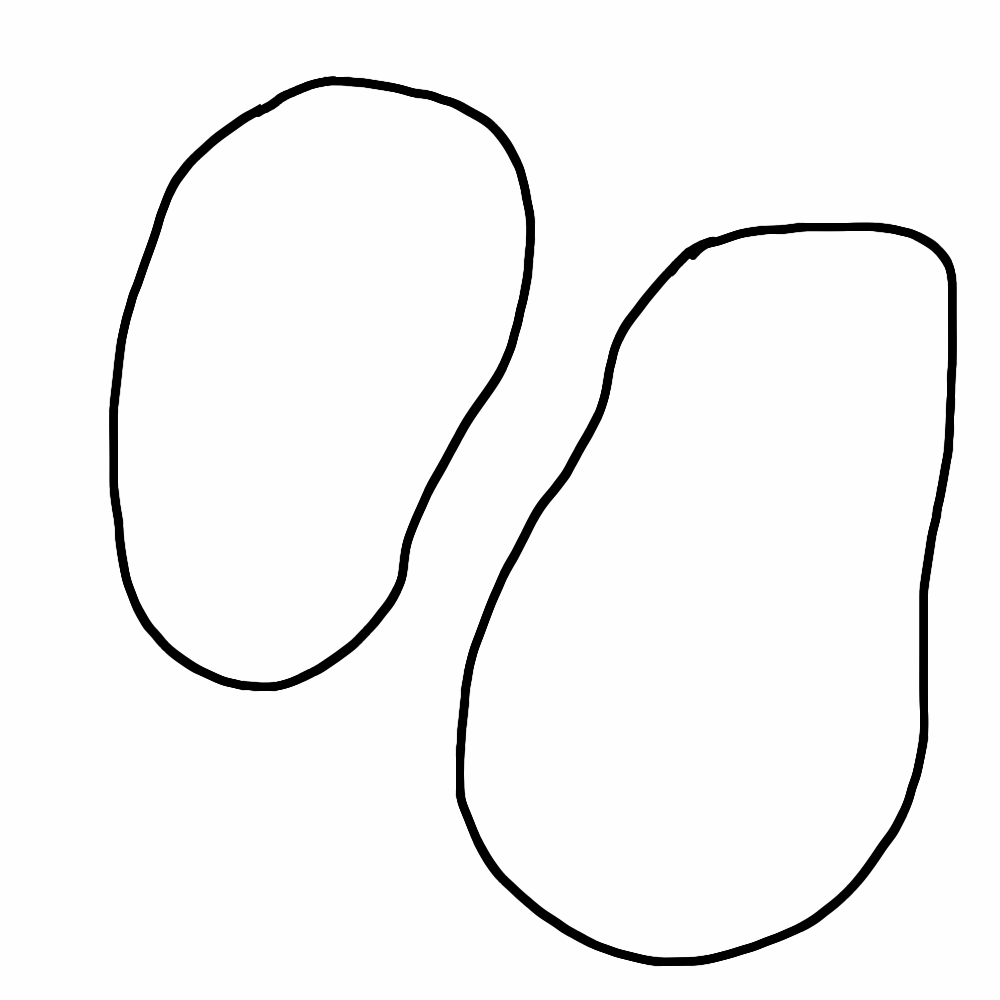
\includegraphics[width=\textwidth]{knotpics/unlink2.png}
        \caption{An Unlink}
    \end{subfigure}
    \quad
    \begin{subfigure}{.3\textwidth}
        \centering
        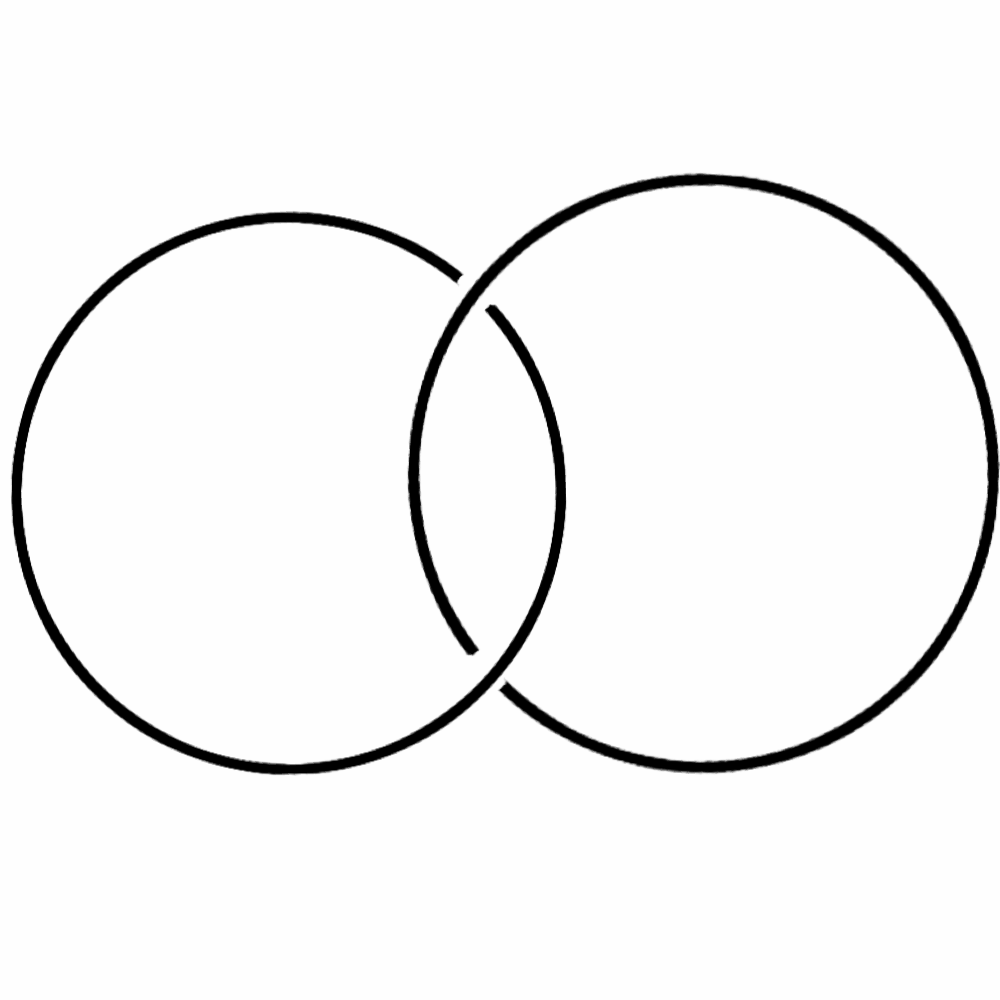
\includegraphics[width=\textwidth]{knotpics/hopf.png}
        \caption{The Hopf Link}
    \end{subfigure}
    \quad
    \begin{subfigure}{.3\textwidth}
        \centering
        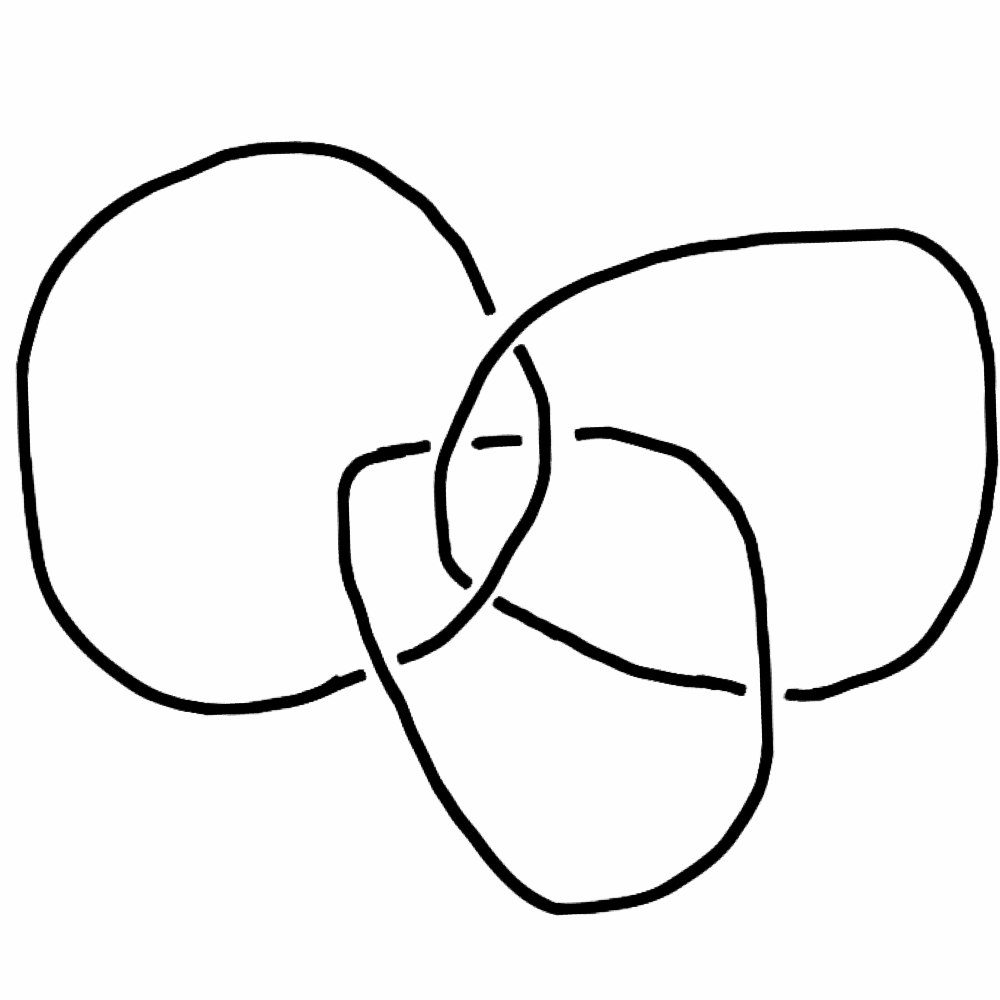
\includegraphics[width=\textwidth]{knotpics/tj3.png}
        \caption{An Anonymous One}
    \end{subfigure}
    \caption{Three Famous Links}
\end{figure}

\clearpage

It is important to be able to recoginze which things are ``true'' links and which are simply knots.

\begin{exercise}
Figure out which of the below is a knot and which is a link but not a knot.
\end{exercise}

\begin{figure}[h]
     \centering
        \begin{subfigure}{.45\textwidth}
        \centering
        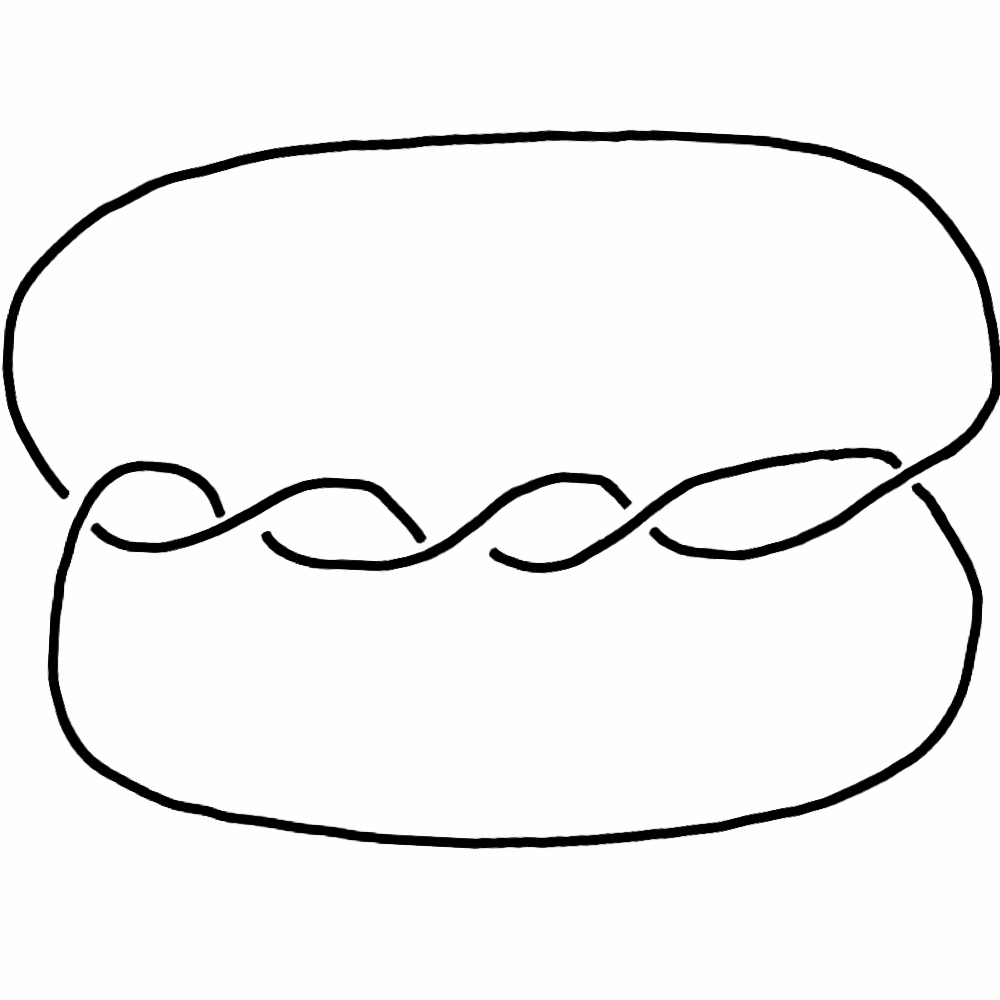
\includegraphics[width=\textwidth]{knotpics/twistknot.png}
        \caption{Link A}
    \end{subfigure}
    \quad
    \begin{subfigure}{.45\textwidth}
        \centering
        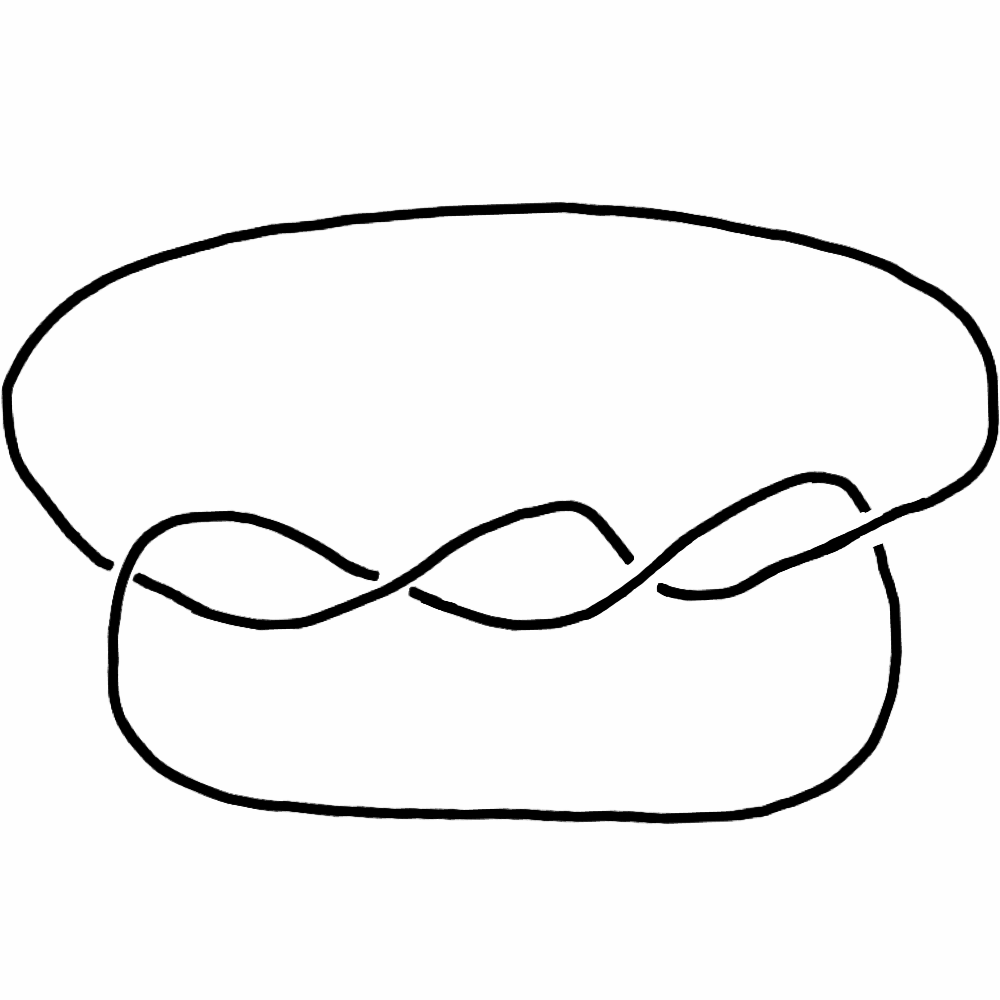
\includegraphics[width=\textwidth]{knotpics/twistlink.png}
        \caption{Link B}
    \end{subfigure}
    \caption{Is either of these a knot?}
\end{figure}

\subsection*{A simple invariant: the number of components}

The way to distinguish the links in the last exercise is by counting the number of connected pieces of string.
Those pieces are called \emph{components}.
Here are some examples of links with the number of components labelled.

\begin{figure}[h]
    \centering
    \begin{subfigure}{.3\textwidth}
        \centering
        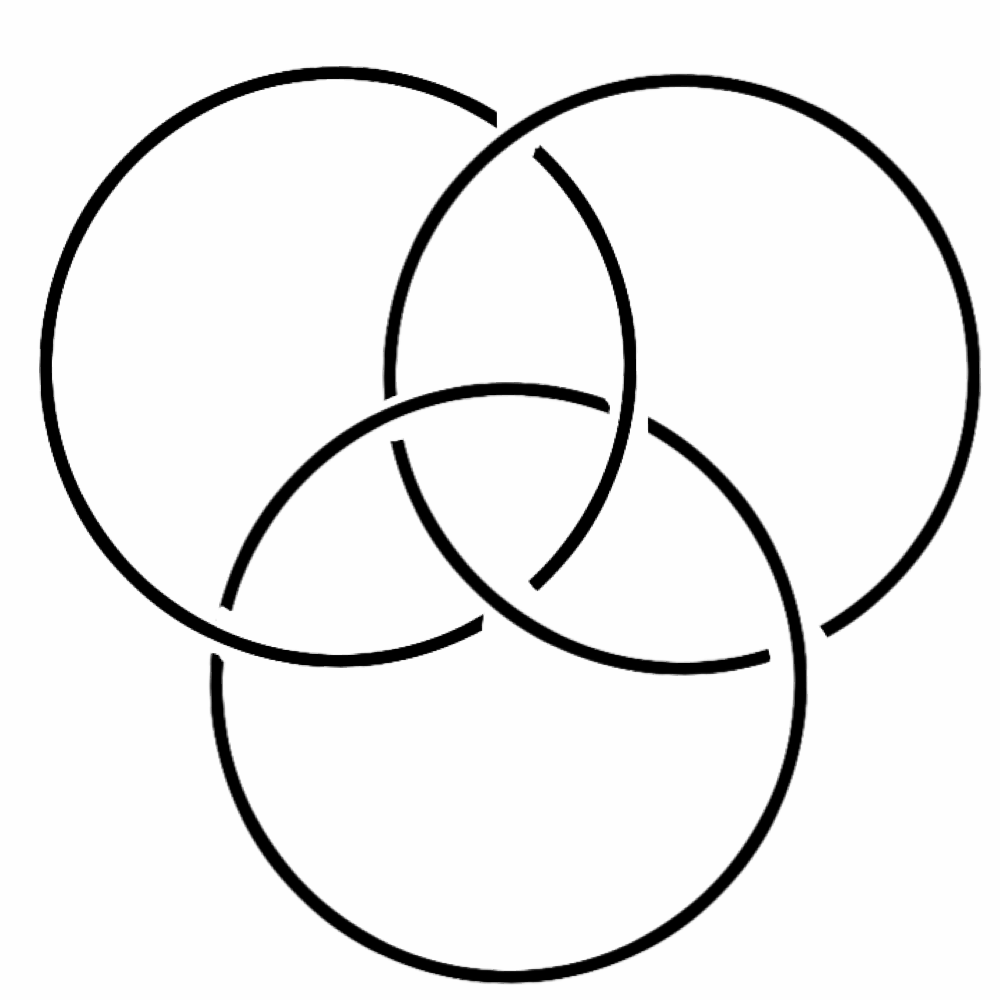
\includegraphics[width=\textwidth]{knotpics/borromean.png}
        \caption{The Borromean Rings:\\ \phantom{space} 3 components}
    \end{subfigure}
    \quad
    \begin{subfigure}{.3\textwidth}
        \centering
        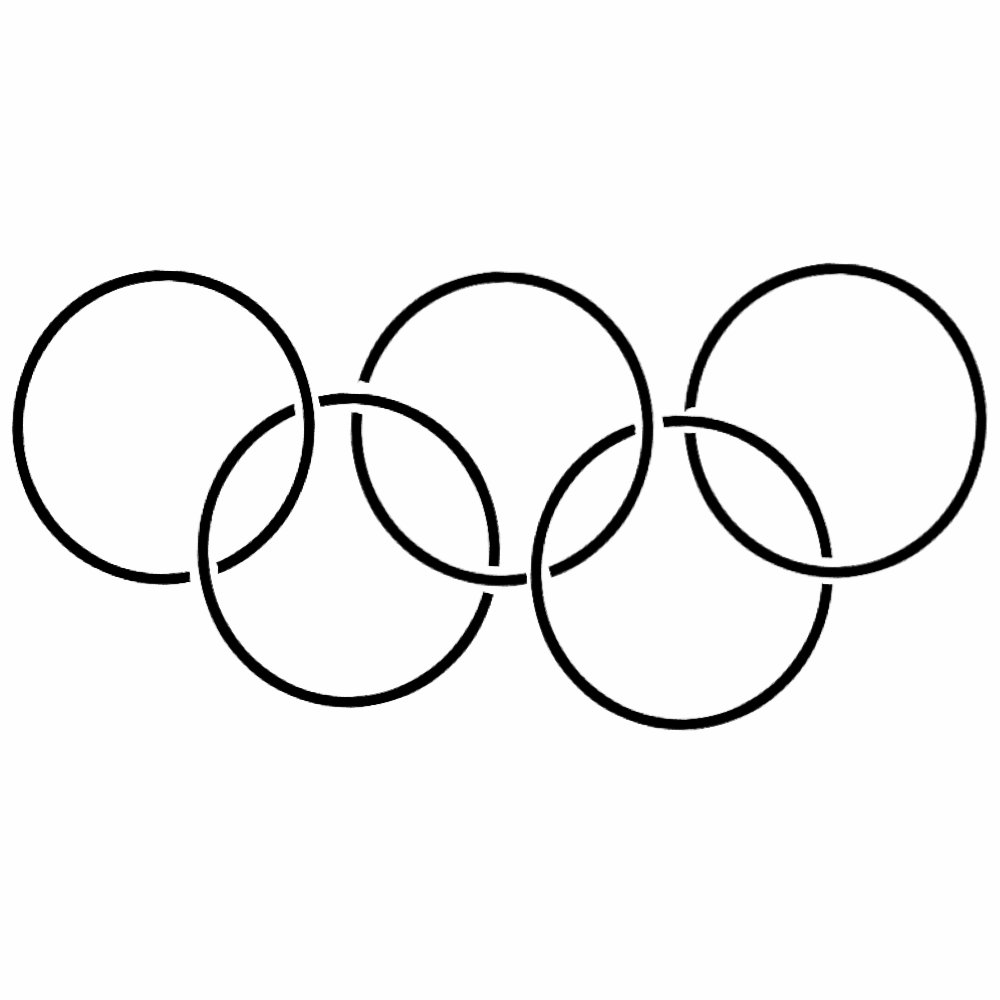
\includegraphics[width=\textwidth]{knotpics/olympic.png}
        \caption{The Olympic Rings:\\ \phantom{space} 5 components}
    \end{subfigure}
    \quad
    \begin{subfigure}{.3\textwidth}
        \centering
        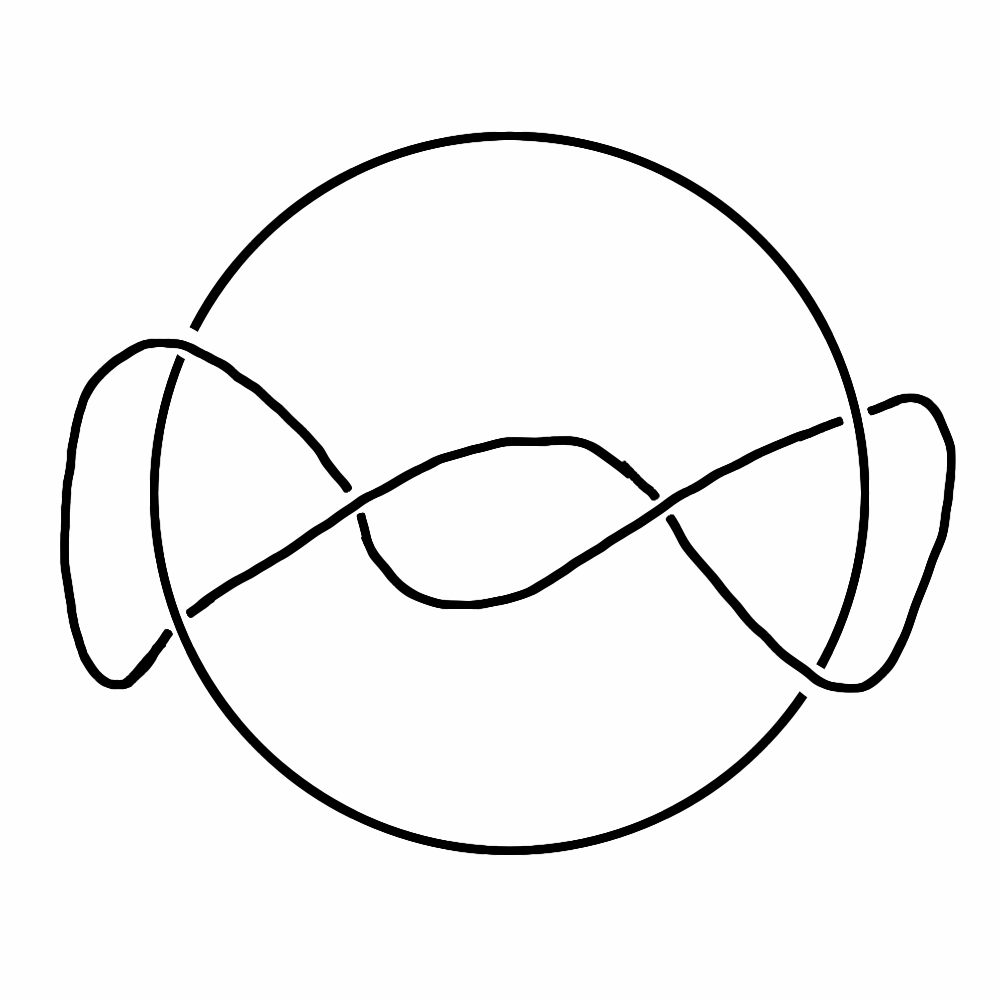
\includegraphics[width=\textwidth]{knotpics/saturntwist.png}
        \caption{An Anonymous One:\\ \phantom{space} 2 components}
    \end{subfigure}
    \caption{Some More Examples}
\end{figure}

The \emph{Borromean Rings} link has a very neat property: if you remove any one of the rings, the other two are no longer linked!
Try it!

The number of components is an invariant of links---no isotopy can change this number.
This makes it a convenient way to distinguish between some links.

\begin{exercise}
Use the number of components to argue that the following links are all distinct from one another:
\begin{compactitem}
\item The figure eight knot.
\item The Hopf Link
\item The Borromean Rings
\end{compactitem}
\end{exercise}

\subsection*{Topological Equivalence of Links}

The natural way to view links as equivalent is the same as that for knots: ambient isotopy.
This means that two links are considered the same if we can move the strings around in space in a way that deforms one link into the other, just like for knots.

One new thing we have is that a link might ``come apart.'' A link is called \emph{splittable} if there is an ambient isotopy which makes the link into a bunch of pieces which are no longer linked.
The pieces might still be knotted, but the individual component knots do not interact with each other.
The unlink above is splittable.

Handling the vast number of possibilities of ambient isotopies is just as big a problem for links as it is for knots.
Fortunately, we have the same hero: Reidemeister Moves. 
The theorem that says we can realize any ambient isotopy of knots by a sequence of Reidemeister moves between planar projections works \emph{exactly the same} for links.
The list of allowed moves is exactly the same, too.

\begin{figure}[h]
     \centering
        \begin{subfigure}{.45\textwidth}
        \centering
        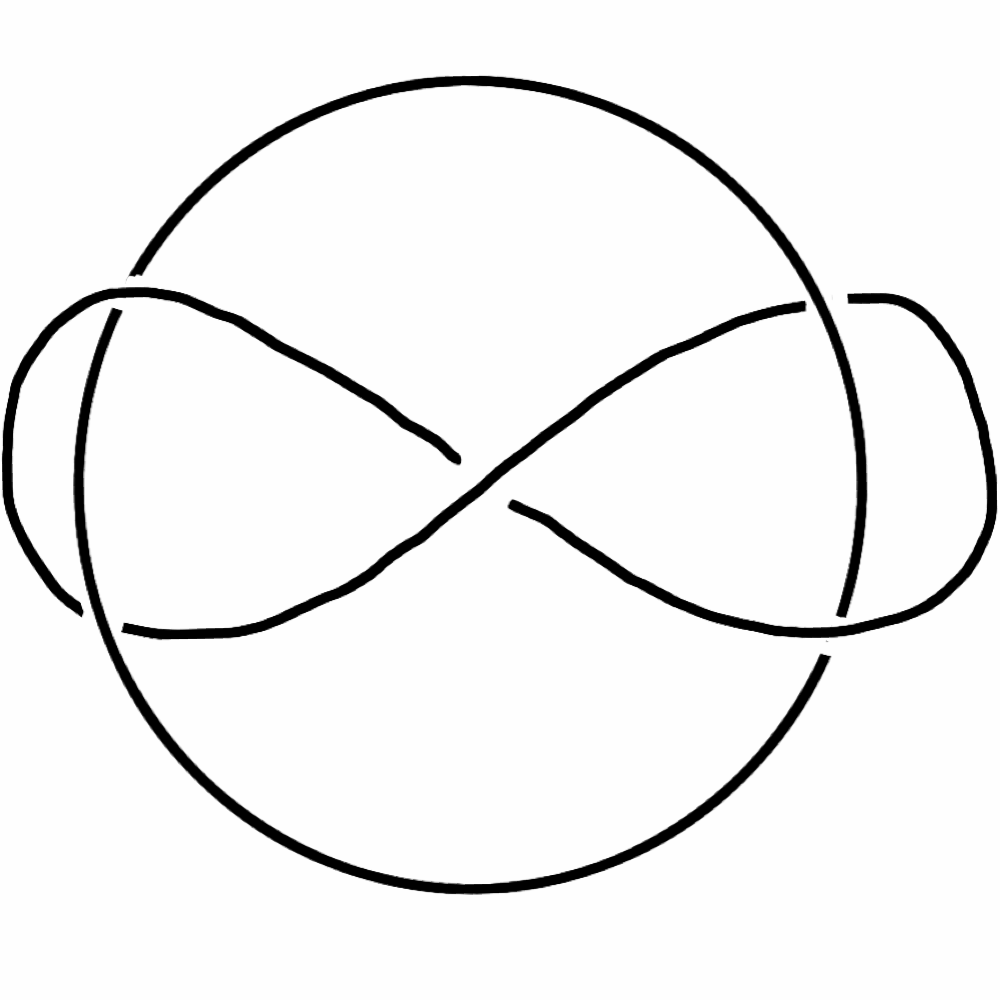
\includegraphics[width=\textwidth]{knotpics/whitehead1.png}
        \caption{The Whitehead link}
    \end{subfigure}
    \quad
    \begin{subfigure}{.45\textwidth}
        \centering
        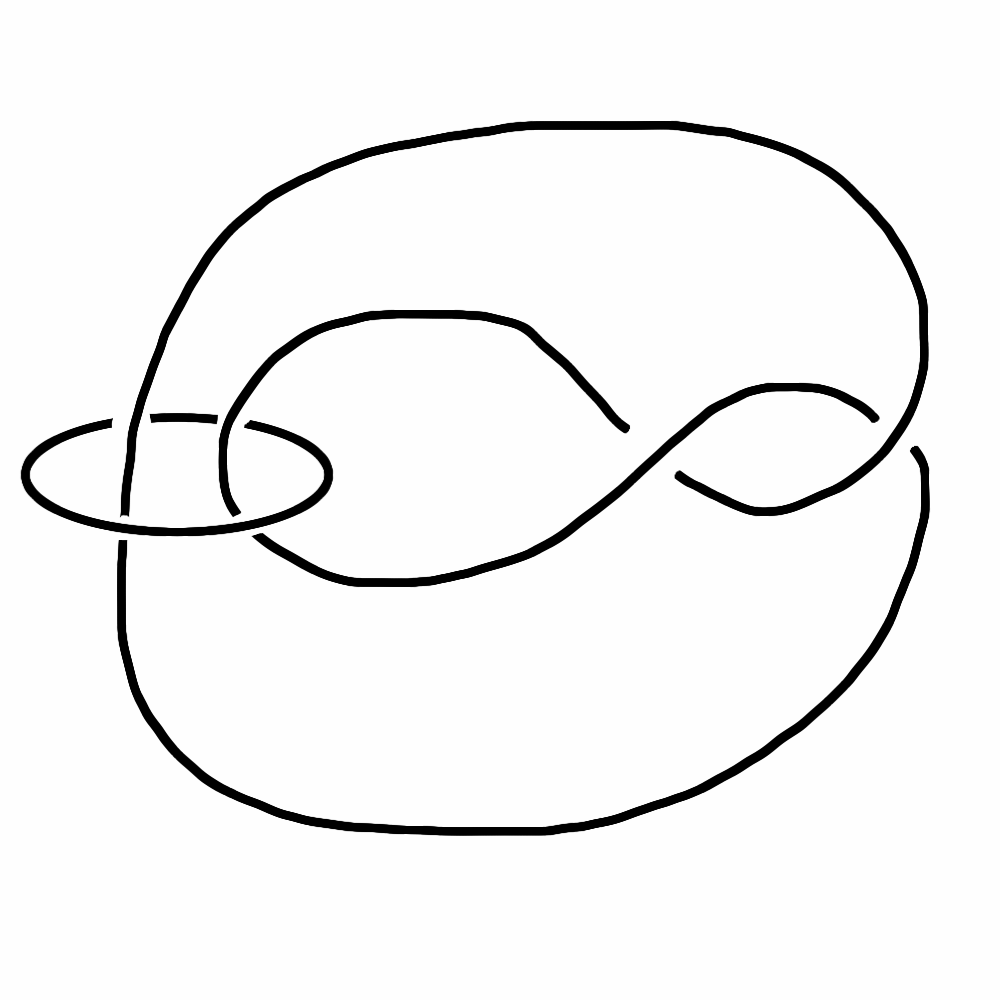
\includegraphics[width=\textwidth]{knotpics/whitehead2.png}
        \caption{Another projection of the Whitehead Link}
    \end{subfigure}
    \caption{Equivalent Links}
\end{figure}


\begin{exercise}
Find a sequence of Reidemeister moves that shows these two planar projections are, in fact, two projections of the same link.
\end{exercise}

\subsection*{Tricolorability for Links}

Another concept that carries over unchanged from knots to links is the notion of tricolorability. 
The rules are exactly the same.
One bit that might happen is that the picture might not be completely determined by one single choice at a crossing, so there might be cases to consider.
So be careful.

Note that the unlink with two (or more) components is tricolorable.
This is different from the simple unknot, which has only one component.
To see this is true for an unlink, take a standard projection consisting of many circles that do not overlap. 
Give each component its own color.
Since there are at least two components, we use at least two colors.
Since there are no crossings, we get that each crossing uses either one or three colors.

\begin{exercise}
Show that the Whitehead link is not tricolorable.
(This means that the Whitehead link is not equivalent to the unlink on two components!)
Can you do this exercise with either planar projection?
\end{exercise}

\begin{challenge}
Is it true that any link with three or more components is tricolorable?
\end{challenge}


\begin{thebibliography}{9}

\bibitem{Adams}
	Colin C. Adams,
	\emph{The Knot Book},
	American Mathematical Society, 
	2004.	


\end{thebibliography}

\end{document}
%sagemathcloud={"zoom_width":100}